\chapter{Punktesortierung in Schachbrettmustern}
\label{sec:schachbrettAlg} 


Um Punktekorrespondenzen in stereoskopischen Bildaufnahmen von zweidimensionalen Schachbrettern zu ermitteln, ist ein Algorithmus entwickelt worden, welcher zuvor detektierte Eckpunkte eines Schachbretts sortiert und eindeutig identifiziert. Jeder Punkt beinhaltet nach der Sortierung die Information in welcher Reihe $j$ und in welcher Spalte $i$ er sich befindet. Jeder Punkt ist somit eindeutig durch die zwei Indizes $i$ und $j$ identifiziert. Dem Sorierungsalgorithmus ist ein Algorithmus zu Detektion der Eckpunkte eines Schachbretts voran geschaltet. Werden beide Algorithmen auf die Stereoaufnahme zweier Schachbretter angewandt, so können korrespondierende Punkte anhand der zugewiesenen Indizes ausgemacht werden. Die Schachbretter können dabei sowohl Kissen- als auch Tonnennverzeichnungen aufweisen und oder perspektivisch verzerrt sein.\\ 



%Das Bild des Schachbretts wird in ein zweidimensionales Koordinatensystem $(A,\alpha)$ mit $\alpha = (j,i)$ gelegt. 

%Als erstes wird ein Startpunkt innerhalb des Schachbretts gesucht. 

Aus den zuvor detektierten Eckpunkten des Schachbretts wird ein Startpunkt ermittelt. Der Startpunkt wird so bestimmt, dass es immer die linke unterste Ecke des Schachbretts ist. Somit ist gewährleistet, dass die Indizes der Eckpunkte beider Bilder gleich sind. Ist der Startpunkt bestimmt, bekommt dieser die Indizes $i = 1$ und $j = 1$. $i$ steht für die jeweilige Reihen in welcher sich ein Punkt befindet und $j$ steht für die jeweilige Spalte. Ist der Startpunkt bestimmt, wird der erste Punkt entlang der unteren Schachbrettkante in $j$-Richtung und der erste Punkt entlang der linken Randkante in $i$-Richtung gesucht. Anhand dieser Punkte lassen sich vom Startpunkt aus Richtungsvektoren definieren. Entlang des Richtungsvektors wird ein Suchbereich definiert. In Abbildung \ref{fig:UebersichtSortierungsAlg} ist dieser Suchbereich als das blaues Dreieck dargestellt. Ist ein neuer Punkt gefunden, so wird der Richtungsvektor anhand des neuen und des vorherigen Punktes neu ausgerichtet. Der dynamische Suchbereich ermöglicht es, dass selbst bei stark verzerrten Schachbrettern, Punkte der einzelnen Reihen und Spalten geordnet werden können, trotz dass diese nicht mehr auf einer Gerade liegen.

%bei denen Punkte nicht mehr auf einer Gerade liegen, einzelnen Reihen und Spalten des Schachbretts geordnet werden.


\begin{figure}[!htb]
	\centering
	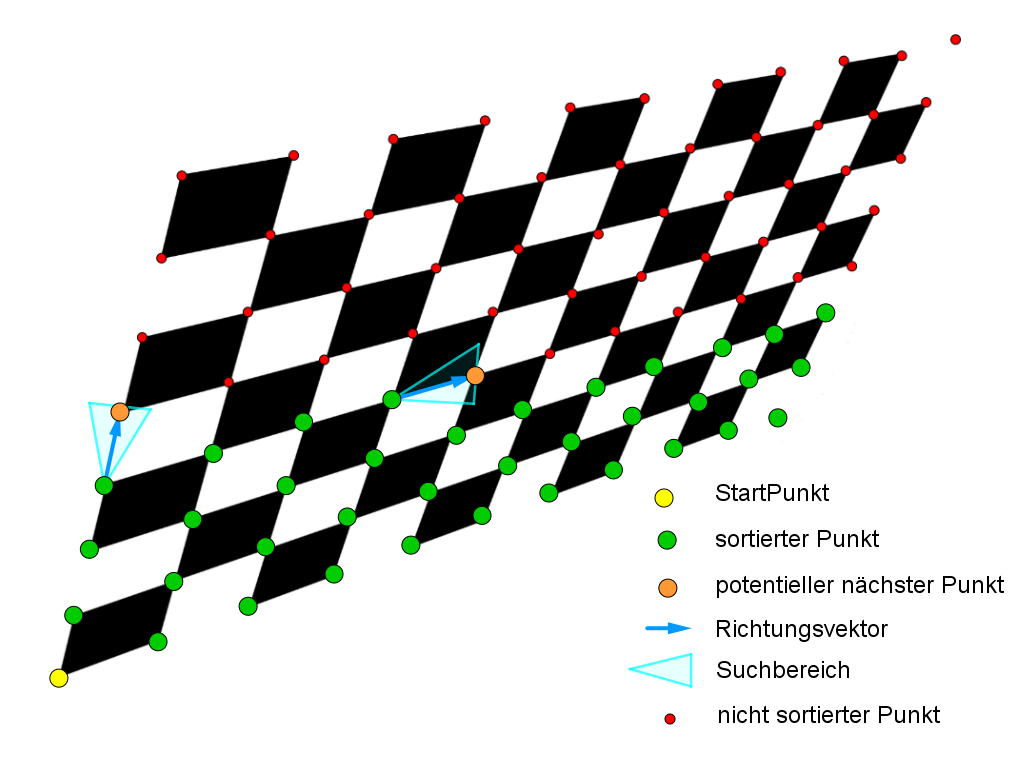
\includegraphics[width=0.8\linewidth]{images/VerzeichnetesSchachbretFunktion.png}
	\caption[Funktionsübersicht des Sortieralgorithmus]{Schematik der Vorgehensweise des Sortieralgorithmus.}
	\label{fig:UebersichtSortierungsAlg}
\end{figure}




\section{Algorithmus zur Sortierung und Indizierung von Schachbretteckpunkten}

Im Folgenden soll der Ablauf des implementierten Sortierungsalgorithmus beschrieben und dessen Funktionsweise an Beispielen von unterschiedlichen Schachbrettern demonstriert werden.\\

Der Soritierungsalgorithmus nimmt eine Liste aus unsortierten Eckpunkten eines Schachbretts entgegen. Von den Punkten in dieser Liste wird eine grobe Vorsortierung vorgenommen. Um das Schachbrett herum wird ein Rahmen definiert. Die Punkte mit der maximalen $y$-Koordinate und der minimalen $y$-Koordinate Begrenzen die oberen und unteren Kanten des Rahmens. Die Punkte mit der minimalen $x$-Koordinate und der Punkt mit der maximalen $x$-Koordinate begrenzen die vertikalen Kanten des Rahmens. In Abbildung \ref{fig:7.1} sind die begrenzenden Kanten in rot um das Schachbrett zu sehen.\\

\begin{figure}[!htb]
	\centering
	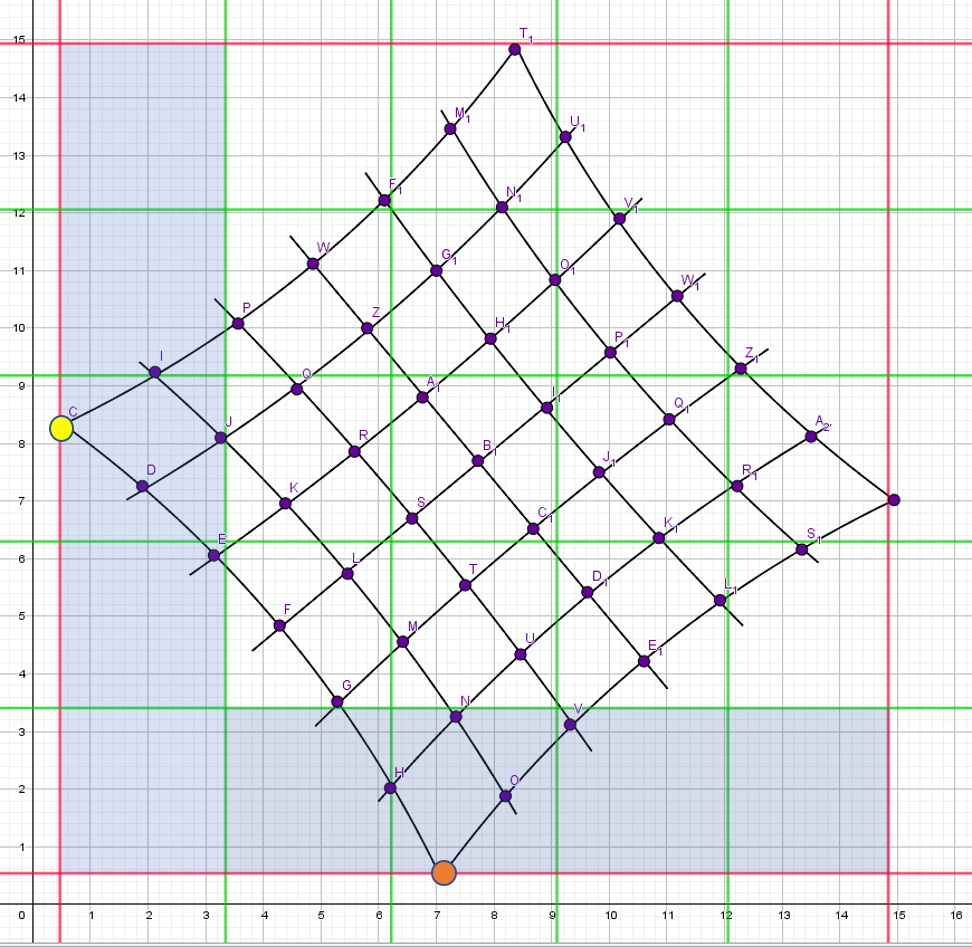
\includegraphics[width=0.6\linewidth]{images/VerzeichnetesSchachbrett_1.png}
	\caption[Startpunktsuche in Schachbretteckpunkten]{Die in blau markierten Bereiche beinhalten die möglichen Startpunkte. Der Bereich entlang der horizontalen $j$- Achse bildet die erste Suchfensterreihe in $i$-Richtung. Der blaue Bereich entlang der vertikalen $i$-Achse bildet die erste Suchfensterreihe in $j$-Richtung. Der gelbe Punkt steht für den Punkt welcher als $VecJ$ bezeichnet wird und der orange Punkt ist derjenige Punkt, welcher als $VecI$ bestimmt wird.}
	\label{fig:7.1}
\end{figure}

Der durch den Rahmen begrenzte Bereich, welcher das gesamte Schachbrett einschließt, wird in mehrere Zellen eingeteilt. Diese werden durchgezählt und mit den Indizes $i$ und $j$ eindeutig bestimmt. $i$ beschreibt die Reihennummer der Zelle und $j$ beschreibt die entsprechende Spalte. In Abbildung \ref{fig:7.1} hätte die Zelle links unten im Eck somit die Indizes $i = 1$ und $j = 1$, die zweite rechts daneben die Indizes $i = 1$ und $j= 2$.\\

In zwei $ConstantArrays$ namens $JSplits$ und $ISplits$ werden die Begrenzungen der Zellen  in $x$- und $y$-Richtung gespeichert. Die Größe und Anzahl der Zellen wird berechnet, indem die Distanz zwischen den vertikalen und horizontalen Kanten des Rahmens durch die gewünschte Anzahl an Zellen geteilt wird. Im nächsten Schritt wird überprüft in welcher Zelle jeder Punkt liegt. Für jeden Punkt wird eine Liste Aus $Associations$ angelegt.  $Associations$ weisen Werten Schlüssel zu. Anhand dieser Schlüssel sind Werte eindeutig identifiziert\cite{Mathematica}. Pro Punkt werden jeweils die $x$- und $y$-Koordinaten sowie die Indizes der Zellen in Schlüssel gespeichert.

\begin{gather*}
	Punkt = \, \{<|Coordx \rightarrow x_u, Coordy \rightarrow y_u, CellI \rightarrow i_u, CellJ \rightarrow j_u |>\} \, .
\end{gather*} \\


Nach der Vorsortierung wird der Startpunkt für die Rekonstruktion des Schachbretts gesucht. Von diesem Startpunkt aus soll das Schachbrettgitter rekonstruiert werden. Alle Punkte innerhalb der Zellen der ersten Reihe mit den Indizes $i = 1$ und der Spalten $j \leq  j_{all}$ und die Punkte der ersten Spalte mit Indizes $i \leq i_{all}$ und $j = 1$ werden als mögliche Startpunkte gekennzeichnet. In Abbildung \ref{fig:7.1} befinden sich die möglichen Startpunkte innerhalb des blau hinterlegten Bereichs.\\


%Die Suche nach einem Startpunkt wird pro $i$- und $j$-Richtung in zwei Abfragen unterteilt.\\
Die jeweiligen horizontalen Zellen $i = 1$ und $j \leq  j_{max}$ werden getrennt von den vertikalen $i \leq i_{all}$ und $j = 1$ untersucht. Innerhalb der horizontalen Zellen wird zunächst nach dem Punkt mit der kleinsten $y$-Koordinate gesucht und als erster möglicher Startpunkt in $VecI$ gespeichert. Danach wird überprüft, ob es einen Punkt gibt, dessen $x$-Koordinate kleiner ist als die des momentan gesetzten $VecI$. Ist dies der Fall so wird noch überprüft, ob dessen $y$-Koordinate kleiner gleich der von $VecI$ plus einem Pufferwert ist. Der Pufferwert wird so definiert, dass die $y$-Koordinate des neuen möglichen $VecI$ zwar größer als die des momentanen sein kann, jedoch eine bestimmte Schwelle nicht übertreten darf, da es sich sonst um einen Punkt der zweiten $i$-Reihe handeln könnte. Für eine mathematische Schätzung des Pufferwerts existieren Ansätze, jedoch wird dieser momentan noch selbstständig gesetzt. In Abbildung \ref{fig:7.1} ist $VecI$ als oranger Punkt abgebildet.\\

Innerhalb des vertikalen Suchbereichs bestehend aus den Zellen  $i \leq i_{all}$ und $j = 1$ wird derjenige Punkt als $VecI$ gesetzt, dessen $x$-Koordinate minimal ist. Im nächsten Schritt wird ein Punkt innerhalb des Bereichs gesucht, dessen $y$-Koordinate kleiner ist als die des momentanen $VecJ$ und dessen $x$-Koordinaten kleiner gleich der $x$-Koordinate von $VecJ$ plus einem Pufferwert ist. Ist so ein Punkt gefunden, wird dieser als neuer $VecJ$ bestimmt. $VecJ$ ist in Abbildung \ref{fig:7.1} als gelber Punkt dargestellt.\\


Je nachdem wie das Schachbrett rotiert ist oder welche Art der Verzerrungen es aufweist, kann es sein dass $VecI$ und $VecJ$ bereits den selben Punkt ergeben, was den Startpunkt $StartPoint$ eindeutig identifiziert, wie es in den Beispielen \ref{fig:Extreme1} oder auch \ref{fig:Extreme5} der Fall ist. Andererseits kann es auch sein, dass $VecI$ und $VecJ$ sich unterscheiden, wie es in Abbildung \ref{fig:7.1} zu sehen ist. In solchen Fällen wurde $VecJ$ als Standard Startpunkt festgelegt. Es kann auch $VecI$ gewählt werden, da in diesen Fällen nicht eindeutig gesagt werden kann, welches die linke unterstes Ecke des Schachbretts ist. Zu beachten ist dabei, dass bei beiden Bilder der selbe Punkt als Startpunkt gewählt wird.\\

Die $Assiciation$-Liste des Startpunktes wird um zwei weitere Schlüssel erweitert. Die Schlüssel $NeighbourI$ und $NeighbourJ$ speichern ab in welcher Reihe $i$ und Spalte $j$ des Schachbrettgitters sich der gefundenen Punkt befindet. Der Startpunkt $StartPoint$ ist dann wie folgt definiert


\begin{gather*}
	\begin{split}
			StartPoint &= \{ <|Coordx \rightarrow x-_u,\, Coordy \rightarrow y_u,\, \\
			&CellI \rightarrow i_u,\, CellJ \rightarrow j_u,\,
			NeighbourI \rightarrow 1, \,NeighbourJ \rightarrow 1 |>\}\, .
	\end{split} 
\end{gather*}
 
Anhand der Schlüssel $NeighbourI$ und $NeighbourJ$, ist die Position des Punktes innerhalb des Schachbrettgitters eindeutig identifiziert. In den Abbildungen \ref{fig:ChessBoardLeftAlg} und \ref{fig:ChessBoardRightAlg} wurde in beiden Bildern alle Punkte abgefragt, deren Schlüssel $NeighbourI = 3$ ist. Die grün gefärbten Punkte liefern das Ergebnis. \\

Der Startpunkt $StartPoint$ wird danach in zwei unterschiedliche Listen geschrieben. Die Liste $SortedPoints$ speichert alle fertig sortierten Punkte. Die Liste $CheckList$ speichert eine verkürzte $Associtaion$-Liste der Punkte, welche nur aus den Schlüsseln $Coordx$ und $Coordy$ besteht. 
\pagebreak
Mit Hilfe der in $Checklist$ gespeicherten Koordinaten eines Punktes, soll bei der weiteren Suche verhindert werden, dass ein Punkt mehrmals in $SortedPoints$ sortiert wird.\\



Nachdem der Startpunkt gefunden ist werden die jeweils nächsten Punkte in $i$- und $j$-Richtung gesucht. Diese Punkte werden dann in die Variablen $NextI$ und $NextJ$ gespeichert. In Abbildung \ref{fig:NextINextJ} ist $NextI$ der violette Punkte und $NextJ$ ist der rote Punkte. \\

Für die Bestimmung von $NextI$ wird zuerst initial $NextI = \, <|Coordx \rightarrow 100 000, Coordy \rightarrow 100 000|>$ gesetzt. Für den Punkt $NextI$ wird die Zelle in welchem sich $StartPoint$ befindet und die jeweiligen Zellen eins darüber und darunter durchsucht. In Abbildung \ref{fig:NextINextJ} ist dieser Bereich um $StartPoint$ gelb hinterlegt. 



\begin{figure}[!htb]
	\centering
	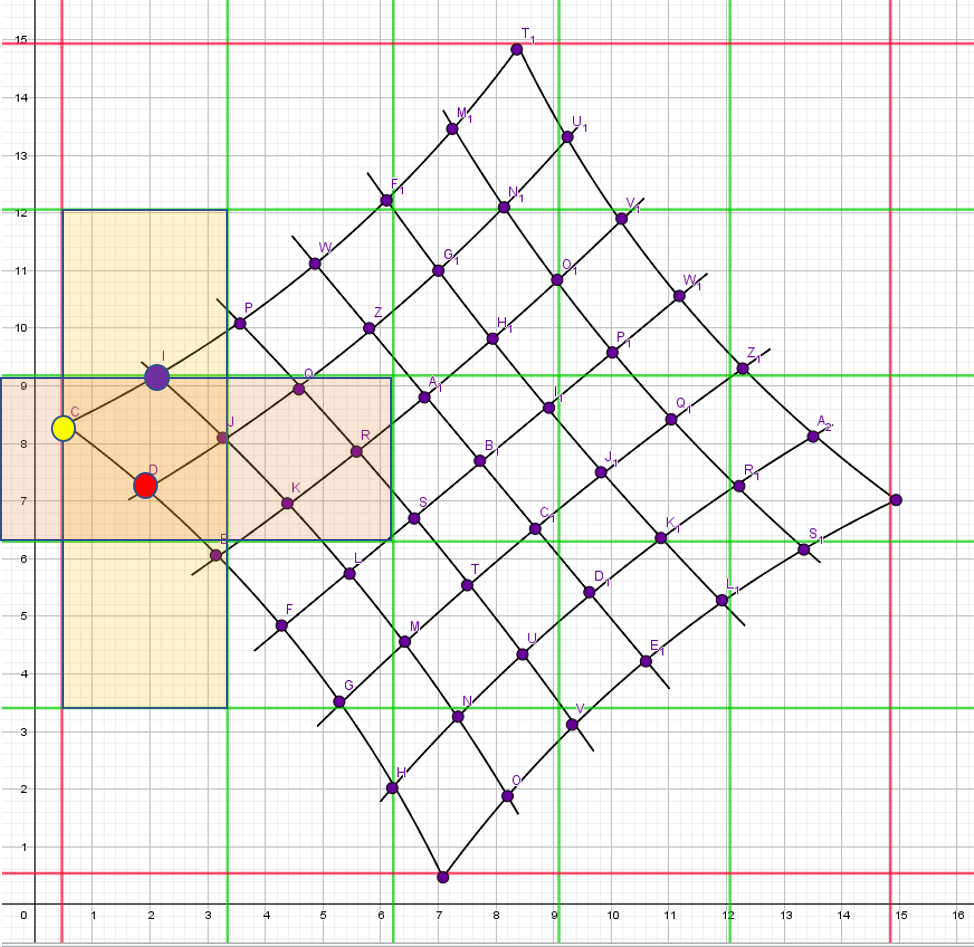
\includegraphics[width=0.6\linewidth]{images/VerzeichnetesSchachbrett_2.png}
	\caption[Bestimmung von Startvektoren]{Der gelb markierte Bereich beinhaltet die für $NextI$ möglichen Punkte. der orange markierte Bereich beinhaltet die für $NextJ$ möglichen Punkte. Der violett gefärbte Punkt ist der gesuchte $NextI$, der rot gefärbte Punkt ist der gesuchte $NextJ$.}
	\label{fig:NextINextJ}
\end{figure}


Innerhalb des Bereichs wird der Punkt mit der zu $StartPoint$ nächst höheren $y$-Koordinate ermittelt. Dieser Punkt wird als vorläufiges $NextI$ festgelegt. Danach wird geprüft, ob das neu bestimmte $NextI$ bereits das letztendliche $NextI$ ist. Dazu werden im gelben Bereich alle Punkte nochmals durchgegangen um zu testen, ob es einen Punkt gibt, welcher einen kleineren $x$-Koordinatenabstand vom Startpunkt besitzt als $NextI$. Gleichzeitig wird geprüft, ob der $y$-Koordinatenabstand vom Startpunkt aus zum neu gefundenen Punkt kleiner ist als der $y$-Koordinatenabstand vom Startpunkt zu $NextI$.  Ist dies der Fall, so wird der Punkt auf den beides zutrifft als neues $NextI$ bestimmt. In Abbildung \ref{fig:FindNextIJ} ist die letzte Abfrage noch einmal grafisch dargestellt. Ist $NextI$ ermittelt, kann dieser Wert im Folgenden nicht mehr als $NextJ$ bestimmt werden. Das kann in Situationen wie in Abbildung \ref{fig:NextINextJ} verhindern, dass für $NextI$ und $NextJ$ der selbe Punkt ermittelt wird.\\

% $NextI$ und $NexrJ$ den selben Punkt darstellen.\\
%
%Um das zu prüfen wird zunächst überprüft ob es innerhalb des gelben Bereichs noch einen Punkt gibt, dessen $x$-Koordinatenabstand vom Startpunkt aus kleiner gleich dem $x$-Koordinatenabstand zwischen dem momentanen $NextI$ zum Startpunkt ist. 

%Gleichzeitig wird geprüft, ob der $y$-Koordinatenabstand zwischen $StartPoint$ und $NextI$ größer ist als der $y$-Koordinatenabstand zwischen einem anderen Punkt innerhalb des Suchbereichs und $StartPoint$.

Die Suche nach dem nächsten Punkt in $j$-Richtung erfolgt nach dem gleichen Prinzip. Für $NextJ$ wird der in Abbildung \ref{fig:NextINextJ} rot hinterlegte Bereich untersucht. Innerhalb des roten Bereichs, wird derjenige Punkt ermittelt der zu $StartPoint$ den nächst höheren $x$-Wert besitzt. Dieser wird dann als vorläufiger $NextJ$ gespeichert. Danach werden alle Punkte im roten Bereich noch einmal durchgegangen und geprüft, ob es einen Punkt gibt, dessen $y$-Koordinatenabstand zum Startpunkt kleiner ist. Gleichzeitig wird abgefragt, ob der $x$-Koordinatenabstand vom Startpunkt aus zum neu gefundenen Punkt kleiner ist als der momentane $x$-Koordinatenabstand vom Startpunkt zu $NextJ$. Die beiden Punkte $NextI$ und $NextJ$ werden dann wie $StartPoint$ um die zwei Schlüssel $NeighbourI$ und $NeighbourJ$ erweitert. Die Punkte sind dann wie folgt definiert und werden in die Liste $SortedPoints$ gespeichert. 


\begin{gather*}
	\begin{split}
		NextI &= \{ <|CoordI \rightarrow i-\text{Koordinate},\, CoordJ \rightarrow j-\text{Koordinat},\, \\
		&CellI \rightarrow i-\text{Zelle},\, CellJ \rightarrow j-\text{Zelle},\,
		NeighbourI \rightarrow 2, \,NeighbourJ \rightarrow 1  |>\}
	\end{split}\\
	\begin{split}
	NextJ &= \{ <|CoordI \rightarrow i-\text{Koordinate},\, CoordJ \rightarrow j-\text{Koordinat},\, \\
	&CellI \rightarrow i-\text{Zelle},\, CellJ \rightarrow j-\text{Zelle},\,
	NeighbourI \rightarrow 1, \,NeighbourJ \rightarrow 2 |>\}
\end{split}
\end{gather*}




\begin{figure}[!htb]
	\centering
	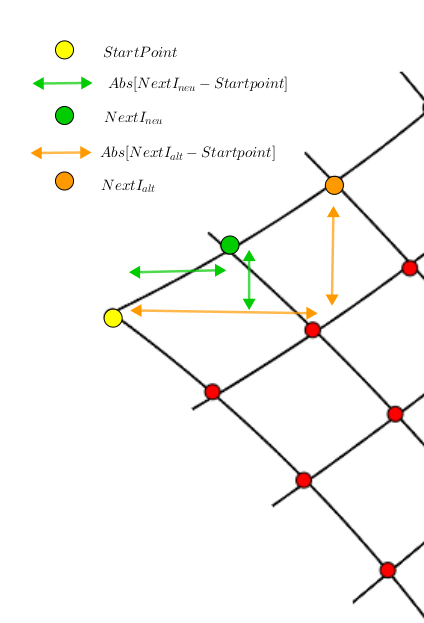
\includegraphics[width=0.5\linewidth]{images/SearchNextI.png}
	\caption[Überprüfung des gefundenen $NextI$]{Um zu überprüfen, ob der momentan $NextI$, in der Abbildung der orange Punkt, wirklich der nächste Punkt ist, wird sein Abstand zum Startpunkt in $j$- und  $i$- Richtung, mit den anderen noch möglichen Punkten verglichen. Gibt es einen dessen beide Abstände kleiner sind, wie beispielsweise der grüne Punkt, so wird dieser zum neuen $NextI$ bestimmt.}
	\label{fig:FindNextIJ}
\end{figure}
\pagebreak


Mit den Punkten $StartPoint$, $NextI$ und $NextJ$ können die ersten Richtungsvektoren in $i$-Richtung mit $NextIDir= NextI - StartPoint$ und $j$- Richtung mit $NextJDir =NextJ-StatPoint$ gebildet werden. Anhand der Richtungsvektoren werden Suchbereiche definiert, in welchen der jeweils nächste Punkt in entsprechender Richtung $i$ oder $j$ gesucht werden soll.\\ 


Für beide Richtungen werden zwei Listen $IList$ und $JList$ angelegt. In den Listen werden jeweils die Punkte der ersten beiden Zellenreihen in $j$- und $i$-Richtung gespeichert. In Abbildung \ref{fig:IListJList} entspricht $IList$ dem vertikalen und $JList$ dem horizontalen blauen Bereich. \\


Der Algorithmus geht dann nach folgendem Schema vor. Zuerst wird die untere Schachbrettkante vervollständigt. Hierzu wird eine Schleife implementiert, welche den im Folgenden beschriebenen Suchvorgang so lange durchgeht, bis keine Punkte mehr gefunden werden. Danach wird der Nächste Punkt der linken Randkante in $i$-Richtung gesucht, von welchem aus wieder die nächste Reihe in $j$-Richtung vervollständigt wird.\\

Für die Vervollständigung der ersten Reihe in $j$-Richtung, wird der Richtungsvektor $NextDirJ$ um einen Puffer erweitert. Dieser Puffer berechnet sich aus einem drittel der Länge von $NextIDir$. Neben dem Richtungsvektor $NextJDir$ wird noch ein Vektor $SearchAreaJ$ definiert, welcher den $i$-Koordinatenabstand zwischen $StartPoint$ und $NextJ$ beinhaltet und den Suchbereich um den Richtungsvektor $NextJDir$ aufspannt. $SearchAreaJ$ wird ebenfalls um einen Pufferwert erweitert. Dieser besteht aus einem drittel der Länge des $i$-Koordinatenabstands von $Startpoint$ zu $NextJ$. In Abbildung \ref{fig:UebersichtSortierungsAlg} ist dieser Puffer als Blauer Kegel um den Richtungsvektor zu sehen. Dieser Kegel definiert den Suchbereich von einem bereits bekannten Punkt zu einem noch unbekannten Punkt. In Abbildung \ref{fig:IListJList} auf dem linken Bild wird der Richtungsvektor $NextJDir$ als Pfeil vom gelben $StartPoint$ zum roten $NextJ$ dargestellt. Die Pfeile welche in $i$-Richtung von $NextJ$ aus ausgehen, bilden die $SearchAreaJ$. Der Bereich den die Vektoren aufspannen bildet den Suchbereich für den auf $NextJ$ folgenden Punkt.

\begin{gather*}
	NextJDir = (NextI - StartPoint) + Puffer\\
	SearchAreaJ = (NextI[CoordI]-StartPoint[CoordI]) + Puffer
\end{gather*}


\begin{figure}[!htb]
	\centering
	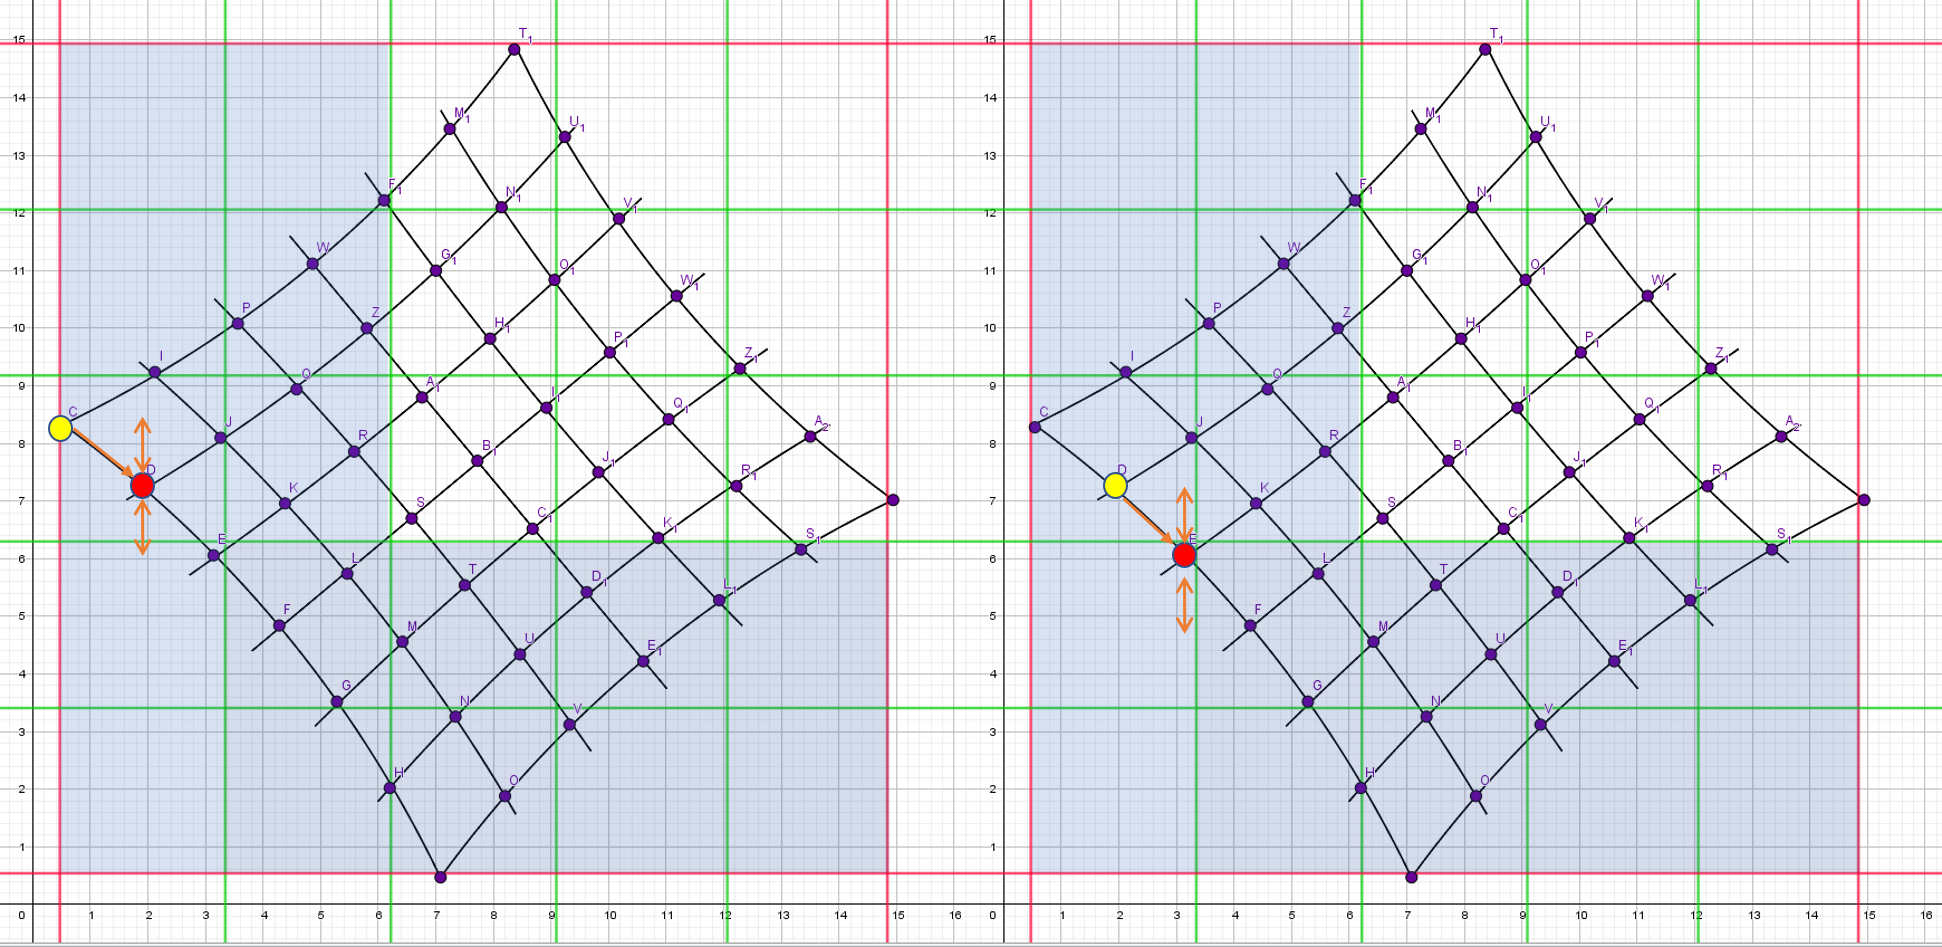
\includegraphics[width=0.8\linewidth]{images/VerzeichnetesSchachbrett_4.png}
	\caption[Suche nach $NextJ$]{Im linken Bild ist der Startpunkt in gelb dargestellt und der bereits gefundenen Punt $NextJ$ ist in rot eingefärbt. Anhand der beiden Punkte wird ein Richtungsvektor definiert und zwei Pufferwerte oberhalb und unterhalb. Diese bilden einen Suchbereich. Der zuvor definierte Suchbereich wird vor $NextJ$ gesetzt und es wird nach einem potentiellen nächsten Punkt in der Reihe gesucht. Ist ein Punkt gefunden, wird $Nextj$ zum neuen $StartPoint$ umdefiniert und der neu gefundene Punkt wird zu $NextJ$.}
	\label{fig:IListJList}
\end{figure}
\pagebreak

Der Ablauf der Schleife zur Vervollständigung einer Reihe wird im Folgenden genauer beschrieben. Der definierte Suchbereich bestehend aus $NextJDir$ und der $SearchAreaJ$ wird vor $NextJ$ platziert. Es werden alle Punkte von $JList$ durchgegangen. Zunächst wird geprüft, ob es einen Punkte innerhalb der Liste gibt, der nicht $StartPoint$ ist und dessen $x$-Koordinate größer ist die $x$-Koordinate von $NextI$. Gleichzeitig wird abgefragt, ob dessen $y$-Koordinate kleiner gleich oder größer gleich der von $NextJ$ ist.\\

Ein solcher Punkt wird als potentieller nächster Punkt weiter überprüft. Es wird sowohl die Distanz $distanceJ$ des Richtungsvektors $NextJDir$ als auch die Distanz von $NextJ$ zum gefundenen potentiellen Punkt berechnet $distanceNextPotPointJ$. Um zu überprüfen, ob der gefundene Punkt innerhalb des Suchbereiches liegt, welcher von $NextJ$ und $SearchArea$ aufgespannt ist, wird der potentielle Punkt auf folgendes getestet. Die $y$-Koordinatenposition des potentiellen Punktes soll zwischen der $y$-Koordinate von $NextJ$ plus dem Wert von $SearchArea$ und der $y$-Koordinate von $NextJ$ minus dem Wert der $SearchArea$ liegen. Des Weiteren darf seine Distanz $distanceNextPotPointJ$ nicht größer werden als $distanceJ$ plus einem Puffer, welcher ein drittel von $distanceJ$ beinhaltet. Zudem darf die Distanz aber auch nicht kleiner sein als die Hälfte von $dinstanceJ$. Als letztes wird mit der $CheckList$ noch sichergestellt, dass der gefundenen Punkt nicht bereits in der $SortedList$ gespeichert wurde.\\

Ist ein solcher Punkt gefunden, so wird $NextJ$ zum neuen $Startpunkt$ und der potentielle Punkt wird zum neuen $NextJ$ deklariert. Es wird der neue Richtungsvektor $NextJDir$ aus dem neuen $StartPoint$ und $NextJ$ berechnet, sowie eine neue $SearchArea$ aus der $i$-Koordinatendifferenz der beiden neuen Punkte $StartPoint$ und $NextJ$. $NextJ$ wird dann noch mit den neuen Schlüsseln $NeighourJ$ und $NeighbourI$ in die Liste $SortedPoints$ gespeichert. Danach beginnt die Schleife mit der Suche nach dem nächsten Punkt in $j$-Richtung. Für jeden weiteren Punkt entlang der Reihe, wird der Bereich der möglichen Punkte neu definiert. Es werden alle Punkte innerhalb der Zellen um den neuen $NextJ$ als neue potentielle Punkte angesehen. Durch diese Begrenzung des Suchbereichs wird der Suchaufwand auf wenige Punkte reduziert. \\

Sind alle Punkte in einer Reihe sortiert, so wird der nächste Punkt $NextI$ entlang der äußeren Kante gesucht. Vom neuen $NextI$ aus startet dann wieder die Schleife, welche die Reihe in $j$-Richtung vervollständigt. Die Suche nach $NextI$ verfährt nach dem selben Verfahren wie $NextJ$ nur wird nach einem neuen gefundenen Punkt für $NextI$ die Funktion für die Vervollständigung der Reihe dazwischen geschaltet.\\

Bevor die Suche entlang einer Reihe oder auch der äußeren Kante als beendet gilt, treten noch zwei Sicherheitsfunktionen in Kraft. Die erste wird als $Saftylist$ bezeichnet. $Saftylist$ sorgt dafür, dass alle Punkte der unteren und der linken Kante des Schachbretts vollständig detektiert werden. Wird beispielsweise kein weiterer Punkt bei der Detektierung der außen Kanten innerhalb der Bereiche von $JList$ oder $IList$ gefunden, so wird der Suchbereich kurzfristig erweitert. Um den letzten gefundenen Punkt innerhalb der Listen werden, sofern vorhanden, alle noch nicht abgesuchten Zellen abgesucht. Gibt es in einer darum liegenden Zelle noch einen Punkt, der in den Suchbereich für den nächsten Punkt fällt, wird dieser noch mit aufgenommen. Die Funktion der $SaftyList$ kommt beispielsweise genau dann zum Einsatz, wenn die Punkte eines Schachbretts wie in \ref{fig:SaftyList} sortiert werden. In der linken Abbildung ist zu sehen, dass der Bereich der $IList$ endet, es aber noch weitere Punkte gibt. Auf der rechten Abbildung ist dann zu sehen, wie der rot hinterlegte Bereich noch hinzugenommen wird, sodass die restlichen Punkte der Kante auch noch gefunden werden.\\

%\begin{figure}[!htb]
%	\centering
%	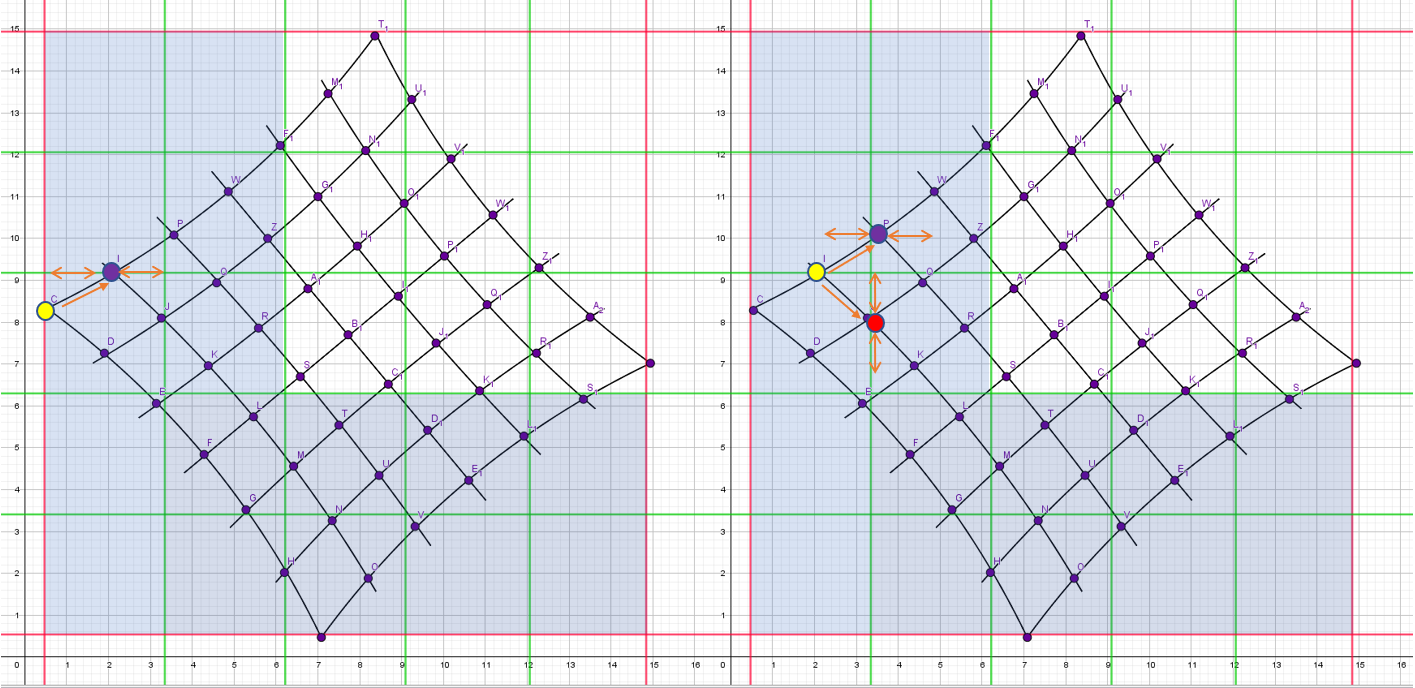
\includegraphics[width=0.8\linewidth]{images/VerzeichnetesSchachbrett_5.png}
%	\caption[Suche nach dem nächsten $NextI$]{Die Suche nach dem nächsten $NextI$ basiert auf dem selben Verfahren wie die Suche nach $NextJ$. Sobald ein neuer $NextI$ gefunden wurde, wird die Reihe in $j$-Richtung vervollständigt, bevor es mit dem nächsten $NextI$ weiter geht}
%	\label{fig:FindNextIPoint}
%\end{figure}

\begin{figure}[!htb]
	\centering
	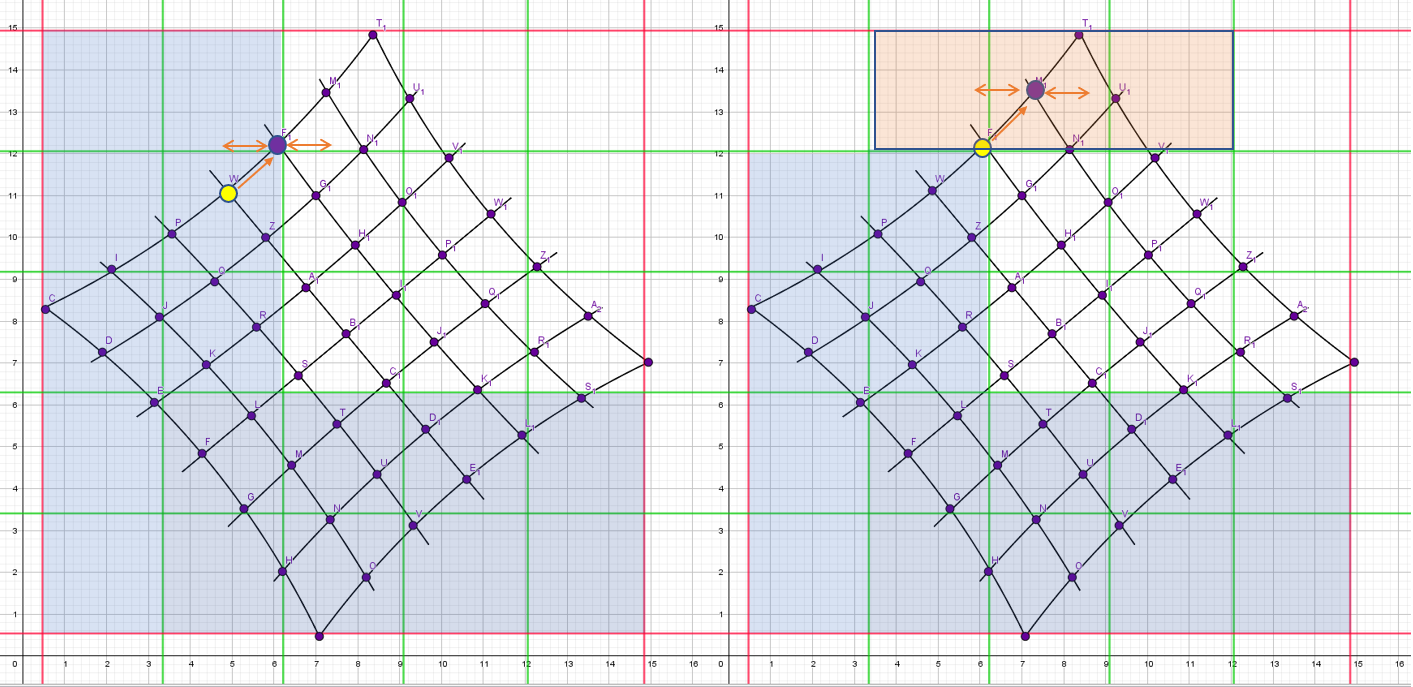
\includegraphics[width=0.8\linewidth]{images/VerzeichnetesSchachbrett_6.png}
	\caption[Sicherheitsfunktion $SaftyList$]{Wird der kein weiterer Punkt innerhalb von $IList$ oder $JList$ gefunden, Wird ein kleiner Bereich, hier in rot hinterlegt, abgesucht, ob es doch noch potentielle nächste Punkte gibt, die aufgrund der Lage des Schachbretts nich in $IList$ oder $JList$ mit enthalten waren.}
	\label{fig:SaftyList}
\end{figure}


Die zweite erwähnte Sicherheitsfunktion ist die $PlaceSyntheticPoint$. Zu Beginn des Sortierungsalgorithmus nimmt dieser eine Punkteliste des voran geschalteten Eckpunktedetektionsalgorithmus entgegen. Bei der Detektion der Eckpunkte, kann es vorkommen, dass Punkte nicht erkannt wurden und somit Lücken im Schachbrettgitter vorhanden sind. Trifft der Sortierungsalgorithmus auf eine solche Lücke, könnte er keinen weiteren Punkt detektieren und würde mit der Suche in der entsprechenden Reihe aufhören. Jedoch können sich hinter der Lücke noch weitere Punkte befinden, welche aber nicht mehr gefunden und sortiert werden. Diese Punkte würden dem entsprechend nicht in der $SortedList$ gespeichert und der Algorithmus würde am Ende die Nachricht ausgeben, dass die Sortierung unvollständig ist.\\

Um dem entgegen zu wirken wurde die Sicherheitsfunktion $PlaceSyntheticPoint$ entwickelt. Sollte vorerst kein Punkt im Suchbereich entdeckt werden, so setzt die Sicherheitsfunktion einen synthetischen Punkt und sucht ausgehend von diesem weiter nach Punkten. Sollte daraufhin ein weiterer Punkt gefunden werden, so bleibt der synthetische Punkt bestehen und die Suche wird normal fortgesetzt. Der synthetische Punkt wird nicht in die Liste $SortedList$ mit aufgenommen, da er später nicht als möglicher korrespondierender Punkt in betrachtet gezogen werden soll. Er dient lediglich dazu alle real vorhandenen Punkte zu finden und richtig zu sortieren. Wird nach dem setzten des synthetischen Punkts kein weiterer Punkt gefunden, gilt die Suche in der Reihe beziehungsweise Spalte für beendet und der synthetische Punkt wird wieder gelöscht. \\


In Abbildung \ref{fig:ChessBoardLeft} und \ref{fig:ChessBoardRight} wird ein Schachbrett aus zwei unterschiedlichen Blickwinkeln dargestellt. Die roten Punkte markieren die Eckpunkte, deren Koordinaten an den Sortierungsalgorithmus übergeben werden. In den Abbildungen \ref{fig:ChessBoardLeftAlg} und \ref{fig:ChessBoardRightAlg} werden alle Punkte, welche in der Liste $SortedPoints$ gespeichert sind in einem Plot ausgegeben. Alle Punkte deren Schlüssel $NeighbourI = 3$ ist, sind in grün dargestellt. Das Ergebnis dieser Abfrage ist in den Abbildungen \ref{fig:ChessBoardLeftAlg} und \ref{fig:ChessBoardRightAlg} zu sehen. Die dargestellten Bilder könnten zwei stereoskopische Abbildungen eines Schachbrettes sein. Der entwickelte Sortierungsalgorithmus kann auf diese Schachbretter angewendet werden und sortiert die Punkte im Schachbrett, sodass korrespondierende Punkte bestimmt werden können und die in den vorherigen Kapiteln beschriebene Szenenrekonstruktion angewandt werden kann. 



%Der entstandene Sortierungsalgorithmus ist also in der Lage aus Bildern zweier Schachbretter gleiche Eckpunkte und somit korrespondierende Punkte zu detektieren. Soll ein einzelner Punkt Abgefragt wollen, so für die Schlüssel $NeighbourI$ und $NeighbourJ$ jeweils ein Wert abgefragt werden.


\begin{figure}[!htb]
	\minipage{0.47\textwidth}
	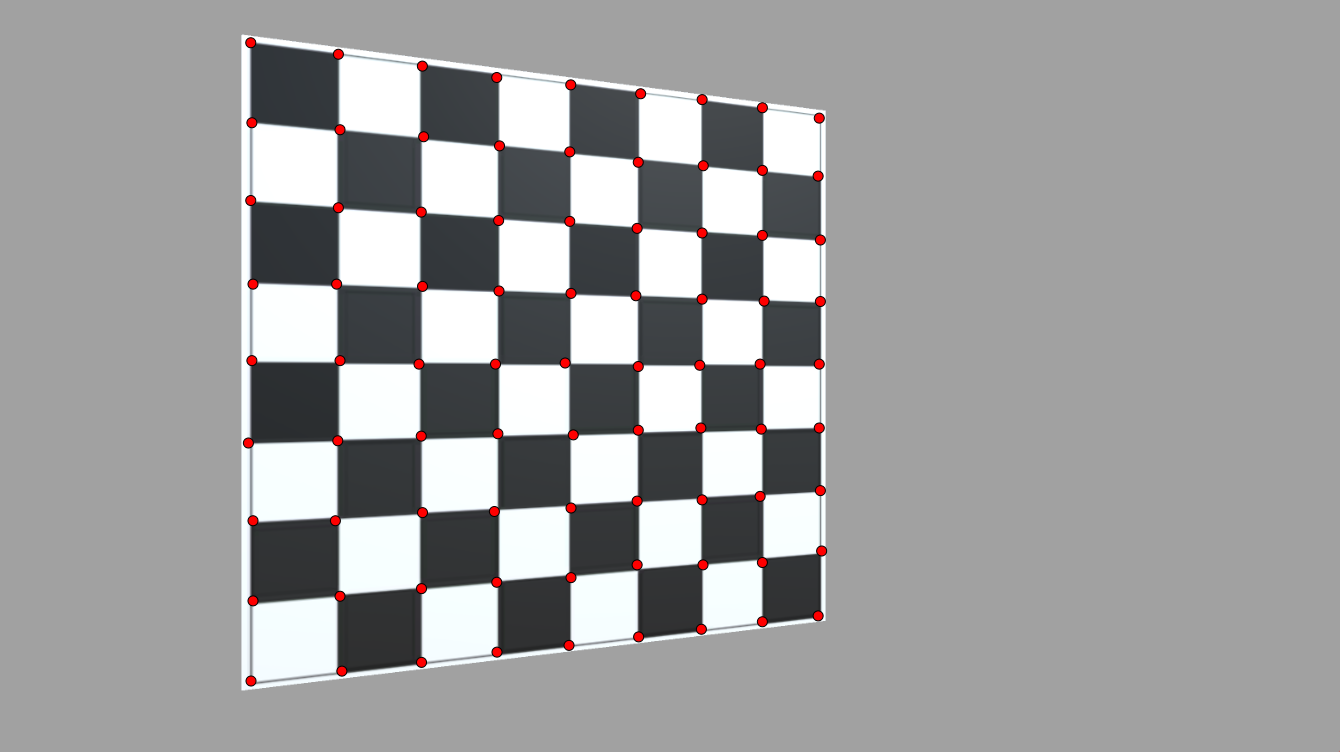
\includegraphics[width=\linewidth]{images/ChessBoardLeft.png}
	\caption[Korrespondezsuche mit Sortierungsalgorithmus: Schachbrett auf linker Seite]{Die Kamera,welche das Schachbrett abbildet steht links versetzt zum Schachbrett und ist rotiert.}
	\label{fig:ChessBoardLeft}
	\endminipage\hfill
	\minipage{0.48\textwidth}
	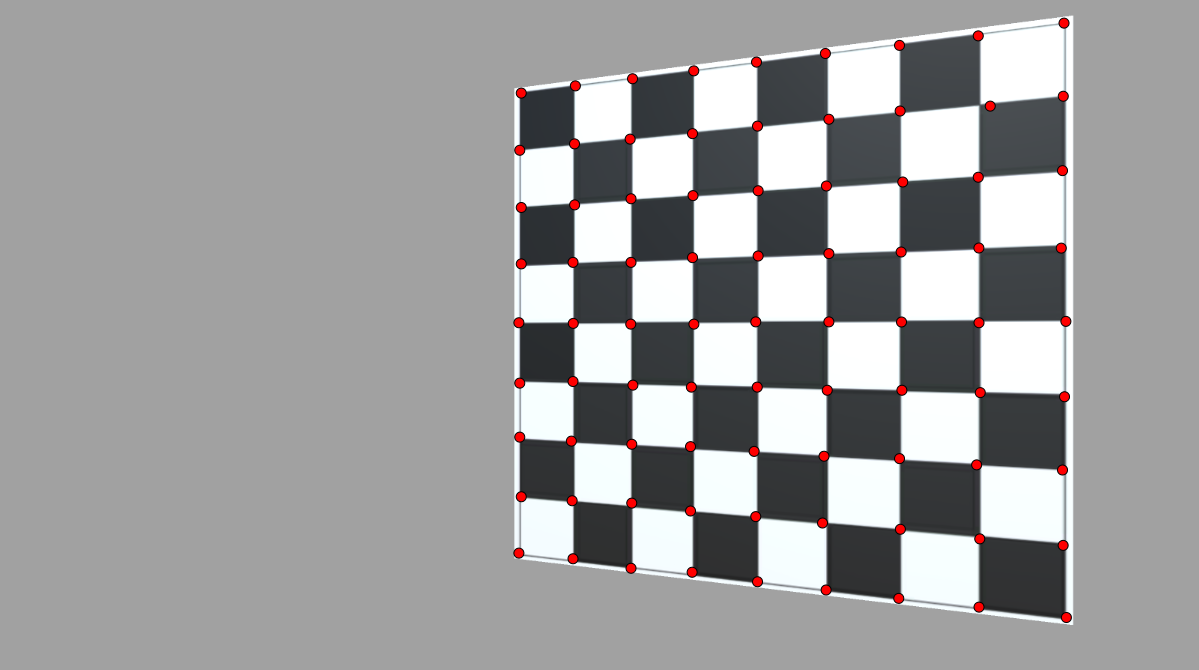
\includegraphics[width=\linewidth]{images/ChessBoardRight.png}
	\caption[Korrespondezsuche mit Sortierungsalgorithmus: Schachbrett auf rechter Seite]{Die Kamera, welche das Schachbrett abbildet steht rechts versetzt zum Schachbrett und ist rotiert.}
	\label{fig:ChessBoardRight}
	\endminipage\hfill
\end{figure}


\begin{figure}[!htb]
	\minipage{0.48\textwidth}
	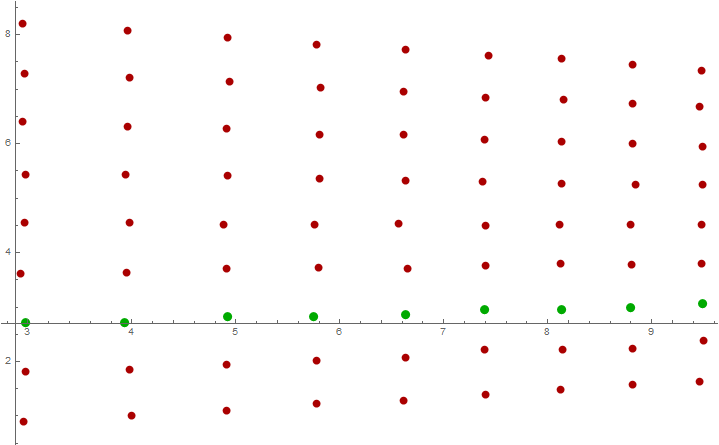
\includegraphics[width=\linewidth]{images/ChessBoardLeftAlg.png}
	\caption[Ergebnis des Sortierungsalgorithmus: Schachbrett auf linker Seite]{Die Abbidlung zeigt das Ergebnis der Sortierung des linken Schachbretts. In grün ist die Reihe an Punkten zu sehen, welche den Schlüssel $NeighbourI = 3$ haben.}
	\label{fig:ChessBoardLeftAlg}
	\endminipage\hfill
	\minipage{0.48\textwidth}
	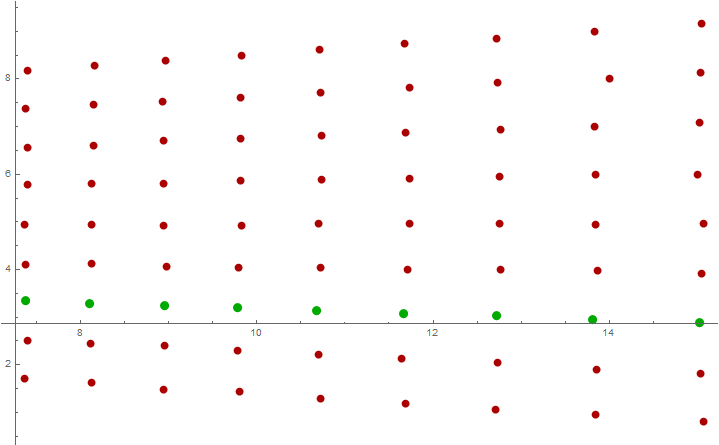
\includegraphics[width=\linewidth]{images/ChessBoardRightAlg.png}
	\caption[Ergebnis des Sortierungsalgorithmus: Schachbrett auf linker Seite]{Die Abbildung zeigt das Ergebnis der Sortierung des rechten Schachbretts. In grün ist die Reihe an Punkten zu sehen, welche den Schlüssel $NeighbourI = 3$ haben.}
	\label{fig:ChessBoardRightAlg}
	\endminipage\hfill
\end{figure}
\pagebreak


\section{Resultate bei stark verzerrten Schachbrettern}
\label{sec:SchachAlgBeispiele}


Der entstandenen Sortierungsalgorithmus wird an stark perspektivisch verzerrten oder durch Bildfehler, wie Verzeichnungen, betroffenen Schachbrettern getestet. Die Möglichkeit herauszufinden, welche Eckpunkte in einem stark verzerrten Bild eines Schachbretts in eine Reihe oder Spalte gehören, kann bei der mathematischen Korrektur von Bildern Anwendung finden. Dies war ein weiterer Grund für die Implementierung dieses Algorithmus und soll in Folgearbeiten weiter studiert werden. \\

% der Bilder von Nutzen sein. Dieser Vorteil war mit ein Grund warum der Algorithmus auf Grundlage von stark verzerrten Schachbrettbilder entwickelt wurde.\\

In den folgenden Beispielen ist jeweils das Originalbild des Schachbretts und daneben die Ausgabe des Algorithmus zu sehen. Der Plot zeigt in rot alle Punkte an, welche in $SortedPoints$ aufgenommen wurden. Alle Punkte, welche als Schlüssel $NeighbourI = 3$ haben, wurden im folgenden grün eingefärbt.


\begin{figure}[!htb]
	\minipage{0.48\textwidth}
	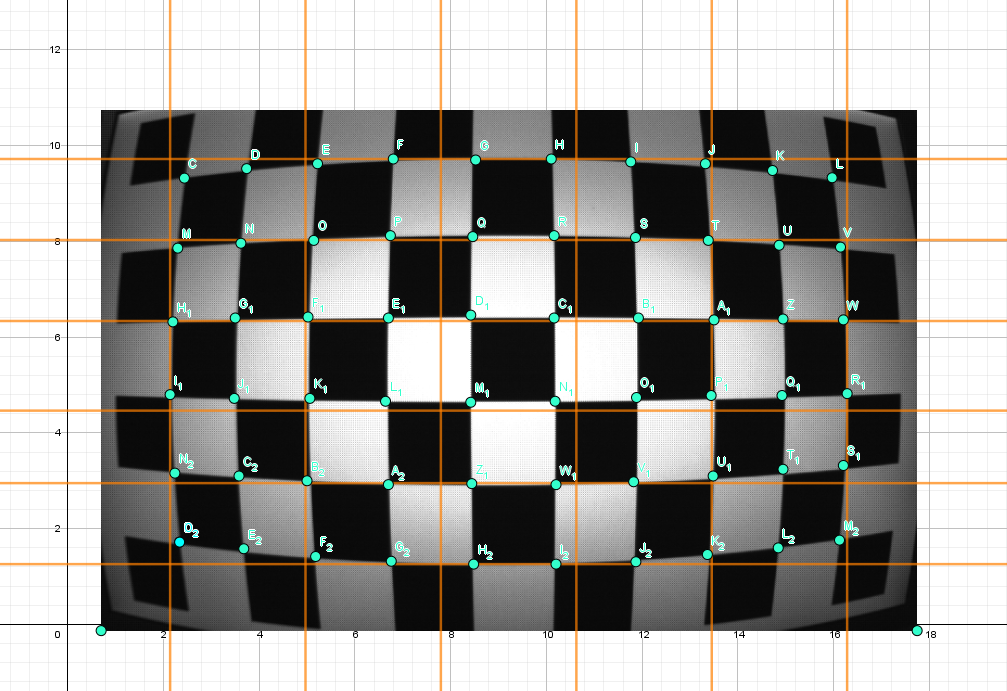
\includegraphics[width=\linewidth]{images/Tonnenverzeichnung.png}
	\caption[Schachbrett mit Tonnenverzeichnung]{Schachbrett mit Tonnenverzeichnung.}
	\label{fig:Extreme1}
	\endminipage\hfill
	\minipage{0.48\textwidth}
	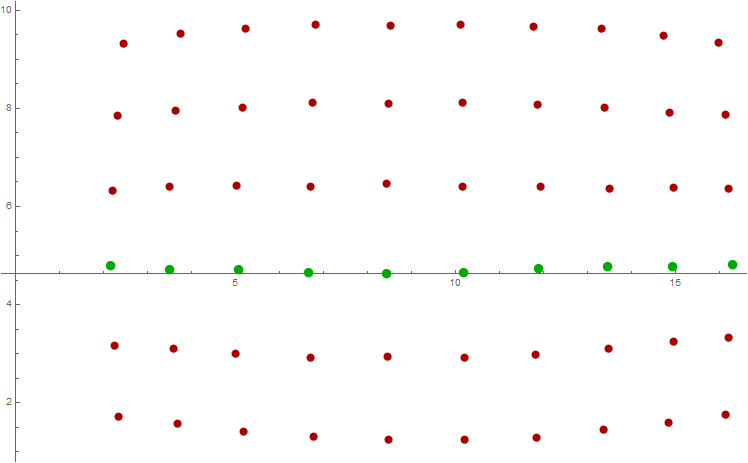
\includegraphics[width=\linewidth]{images/AlgTonnenverzeichnung.png}
	\caption[Sortierte Punkte eines Schachbretts mit Tonnenverzeichnung]{Ergebnis des Sortierungsalgorithmus.}
	\label{fig:Extreme2}
	\endminipage\hfill
\end{figure}

\begin{figure}[!htb]
	\minipage{0.45\textwidth}
	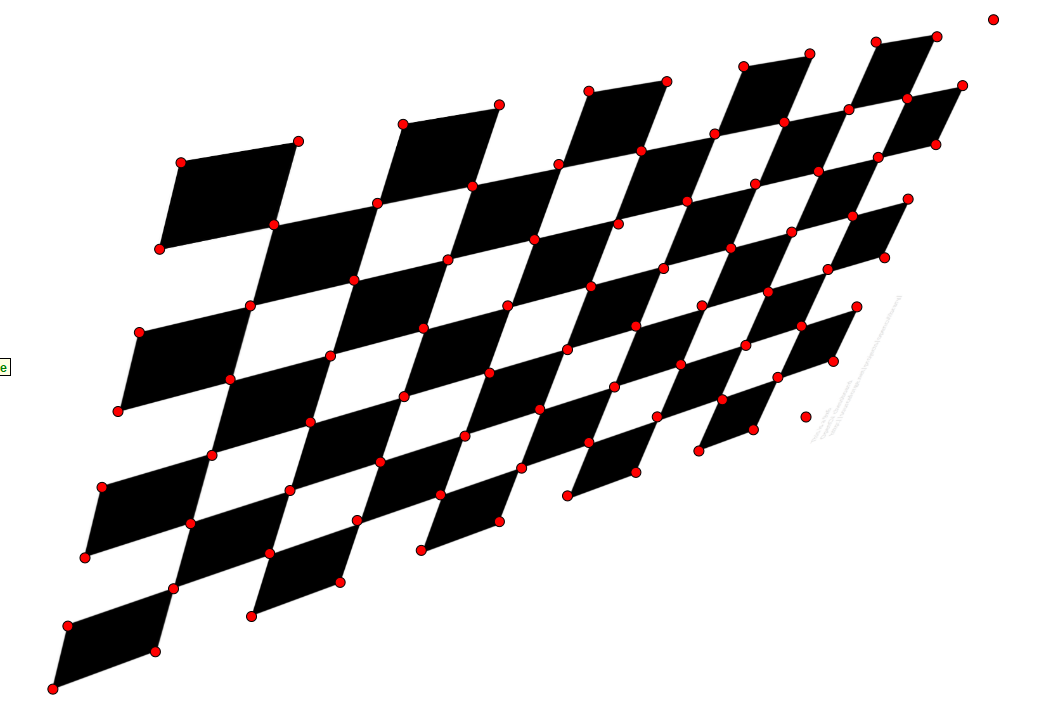
\includegraphics[width=\linewidth]{images/perspektivisch.png}
	\caption[Perspektivisch stark verzerrtes Schachbrett]{Perspektivisch stark verzerrtes Schachbrett.}
	\label{fig:Extreme3}
	\endminipage\hfill
	\minipage{0.49\textwidth}
	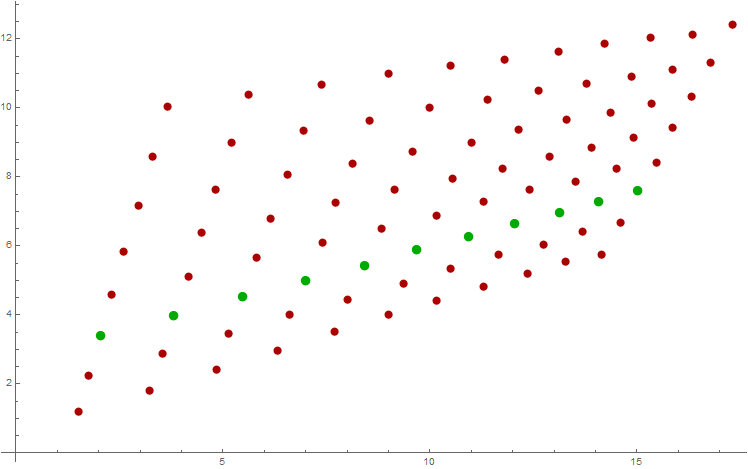
\includegraphics[width=\linewidth]{images/AlgPerspektifisch.png}
	\caption[Sortierte Punkte eines perspektivisch verzerrten Schachbretts]{Ergebnis des Sortierungsalgorithmus.}
	\label{fig:Extreme4}
	\endminipage\hfill
\end{figure}


\begin{figure}[!htb]
	\minipage{0.48\textwidth}
	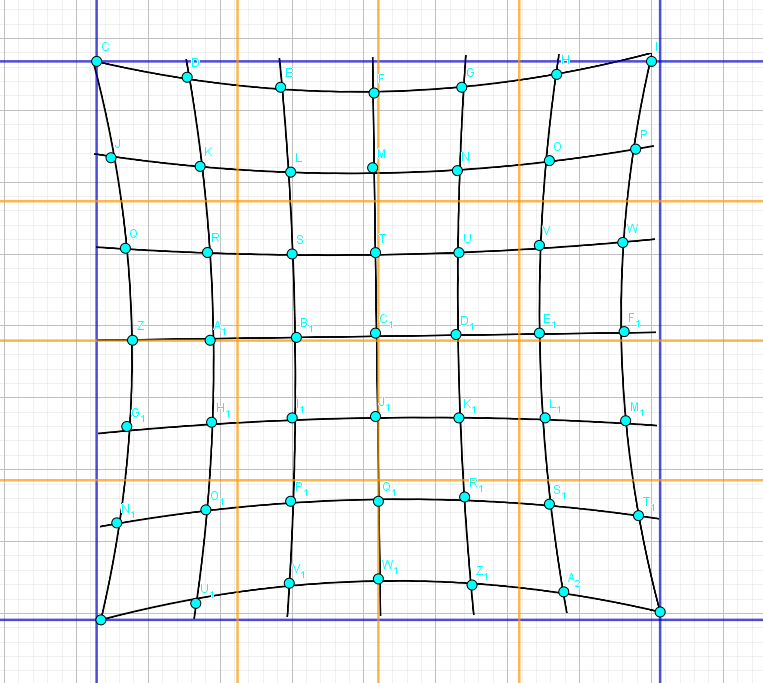
\includegraphics[width=\linewidth]{images/KissenVerzeichnung.png}
	\caption[Schachbrett mit Kissenverzeichnung]{Schachbrett mit Kissenverzeichnung.}
	\label{fig:Extreme5}
	\endminipage\hfill
	\minipage{0.50\textwidth}
	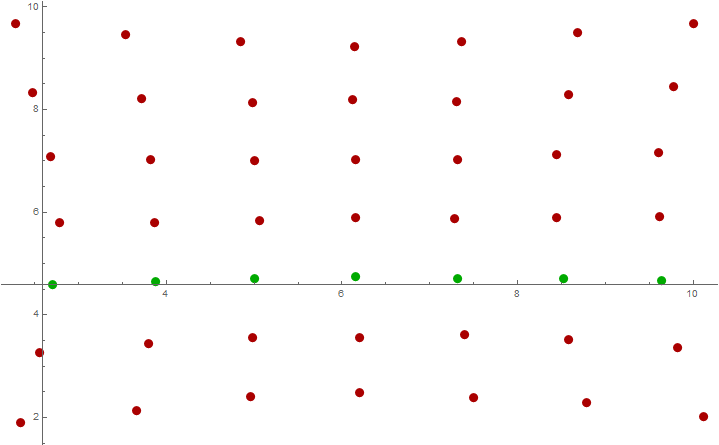
\includegraphics[width=\linewidth]{images/AlgKissen.png}
	\caption[Sortierte Punkte eines Schachbretts mit Kissenverzeichnung ]{Ergebnis des Sortierungsalgorithmus.}
	\label{fig:Extreme6}
	\endminipage\hfill
\end{figure}

\begin{figure}[!htb]
	\minipage{0.48\textwidth}
	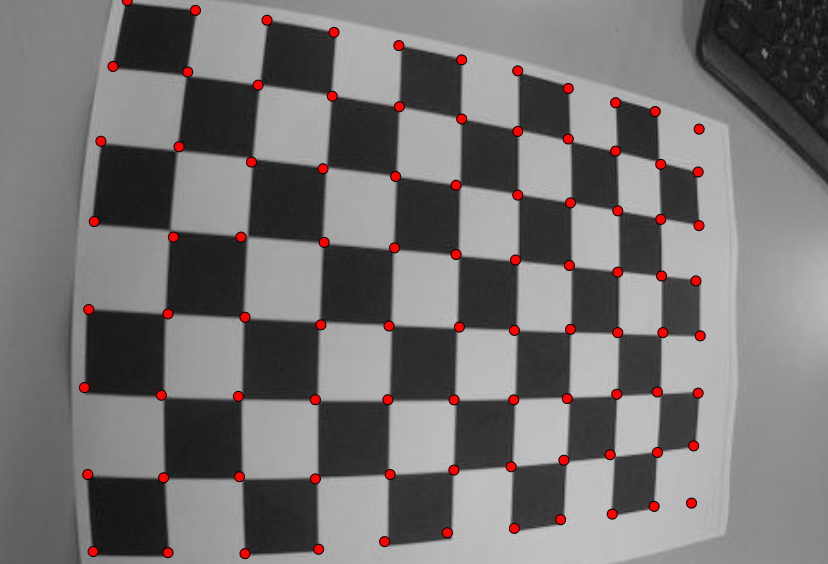
\includegraphics[width=\linewidth]{images/Tonnenverzeichnung_Perspektivisch.png}
	\caption[Perspektivisch verzerrtes Schachbrett mit Tonnenverzeichnung]{Perspektivisch verzerrten Schachbrett mit Tonnenverzeichnung.}
	\label{fig:Extreme7}
	\endminipage\hfill
	\minipage{0.48\textwidth}
	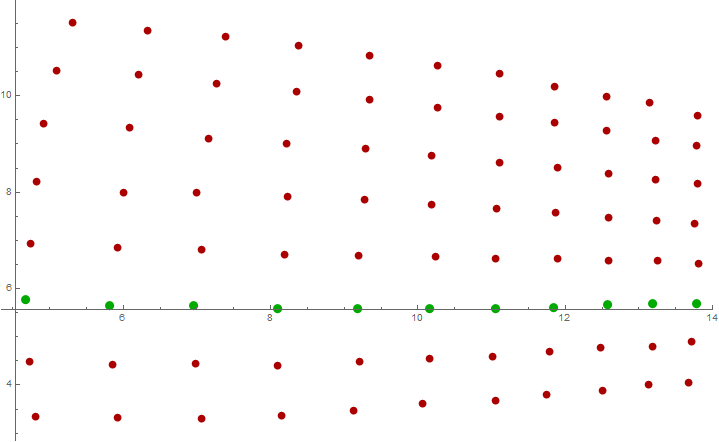
\includegraphics[width=\linewidth]{images/Tonnenverzeichnung_Perspektivisch_Alg.png}
	\caption[Sortierte Punkte eines perspektivisch verzerrten Schachbretts mit Tonnenverzeichnung]{Ergebnis des Sortierungsalgorithmus.}
	\label{fig:Extreme8}
	\endminipage\hfill
\end{figure}

\begin{figure}[!htb]
	\minipage{0.48\textwidth}
	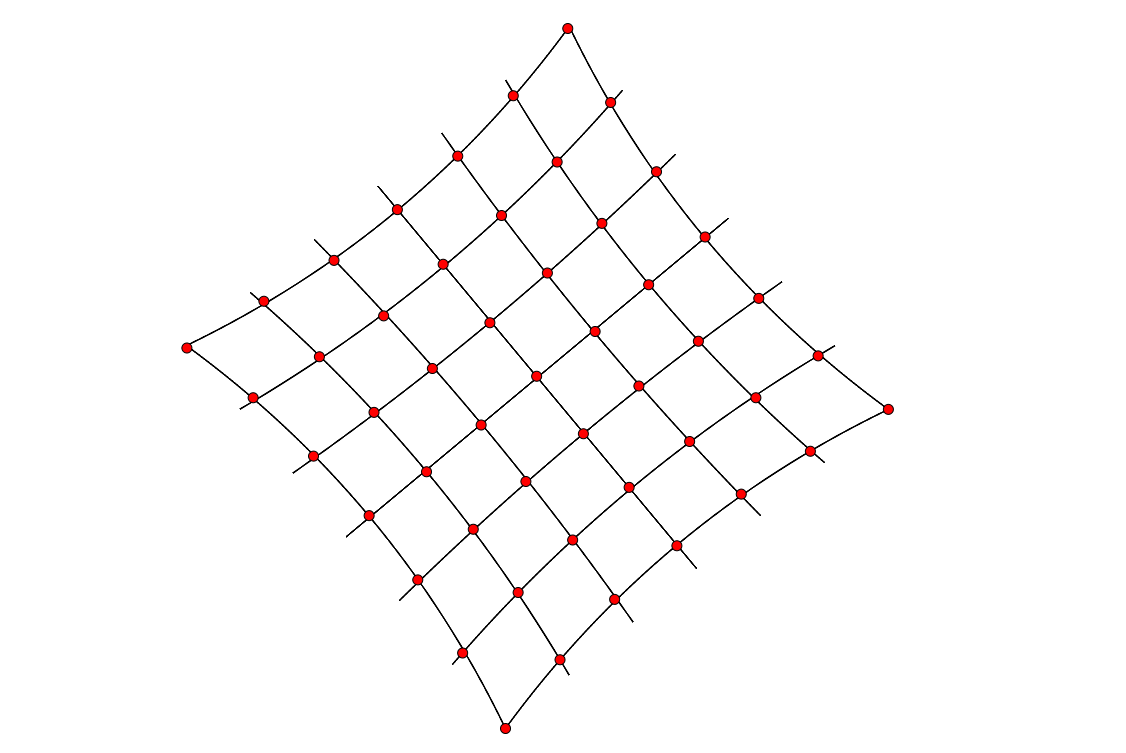
\includegraphics[width=\linewidth]{images/extrBsp.png}
	\caption[Rotiertes Sachbrett mit Kissenverzeichnung]{Rotiertes Sachbrett mit Kissenverzeichnung.}
	\label{fig:Extreme9}
	\endminipage\hfill
	\minipage{0.48\textwidth}
	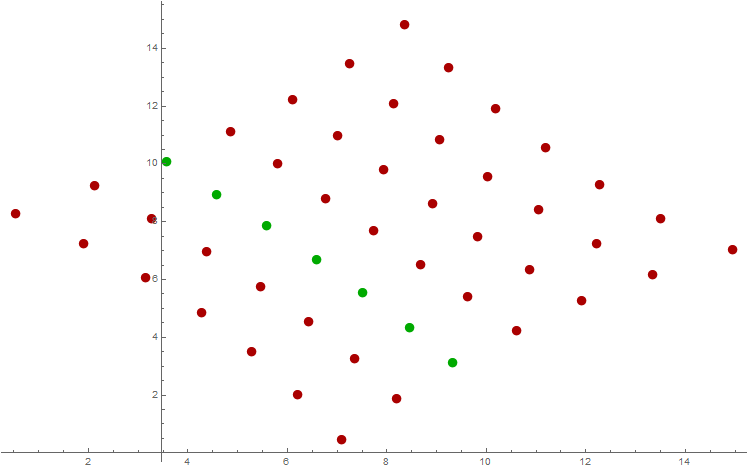
\includegraphics[width=\linewidth]{images/AlgExtrBsp.png}
	\caption[Sortierte Punkte eines rotierten Schachbretts mit Kissenverzeichnung]{Ergebnis des Sortierungsalgorithmus.}
	\label{fig:Extreme10}
	\endminipage\hfill
\end{figure}


%\section{Modulübersicht}
%
%
%\begin{minipage}{\linewidth}
%	\centering
%	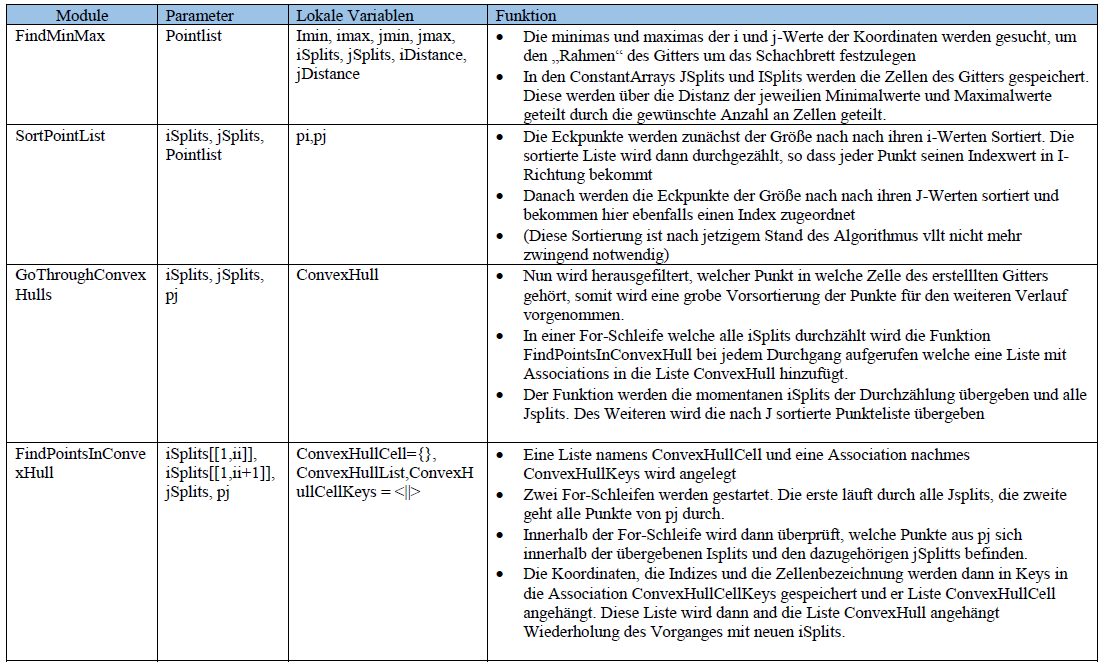
\includegraphics[width=1\linewidth]{images/KD1.png}
%	\captionof{figure}{Klassendiagramm}
%\end{minipage}
%\begin{minipage}{\linewidth}
%	\centering
%	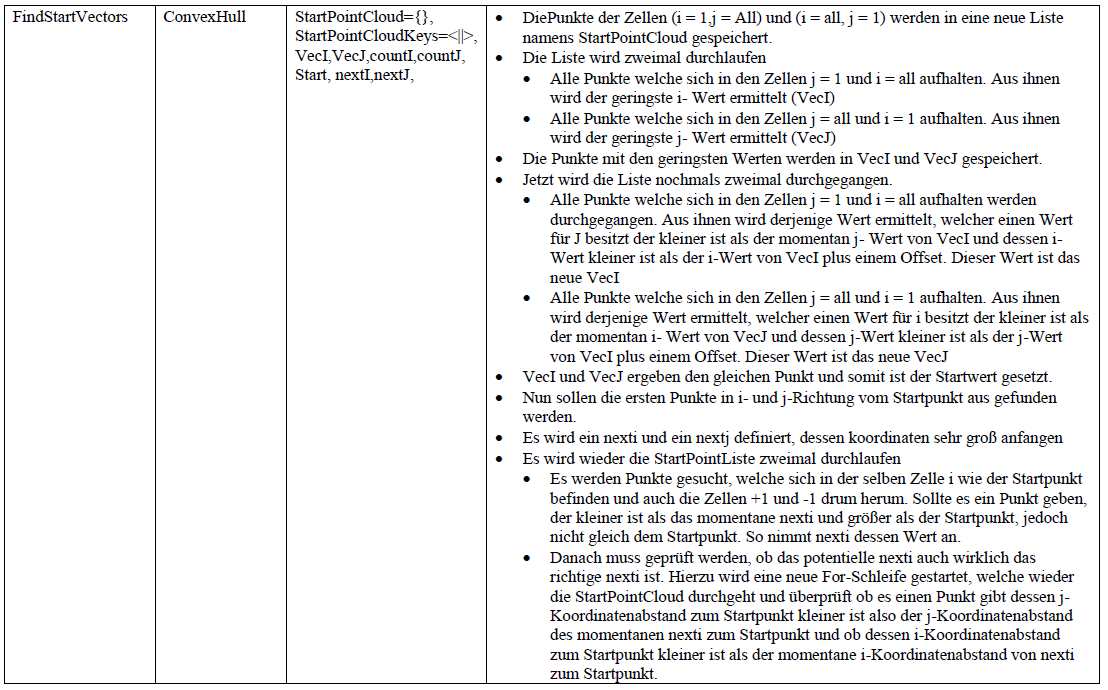
\includegraphics[width=1\linewidth]{images/KD2.png}
%	\captionof{figure}{Klassendiagramm}
%\end{minipage}
%\begin{minipage}{\linewidth}
%	\centering
%	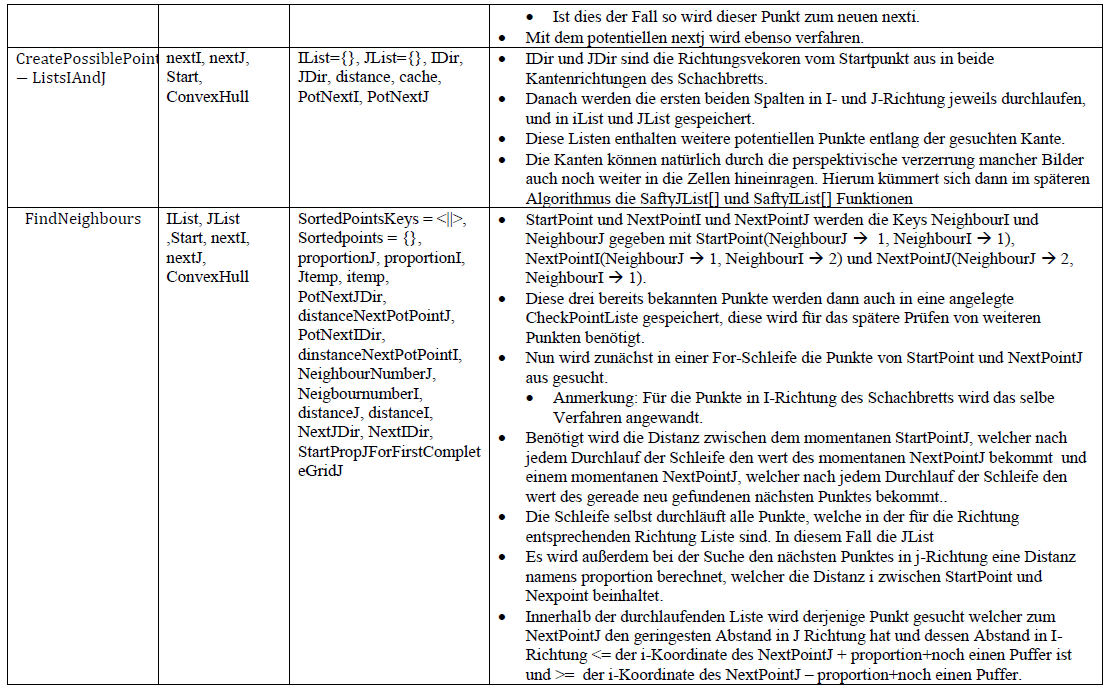
\includegraphics[width=1\linewidth]{images/KD3.png}
%	\captionof{figure}{Klassendiagramm}
%\end{minipage}
%\begin{minipage}{\linewidth}
%	\centering
%	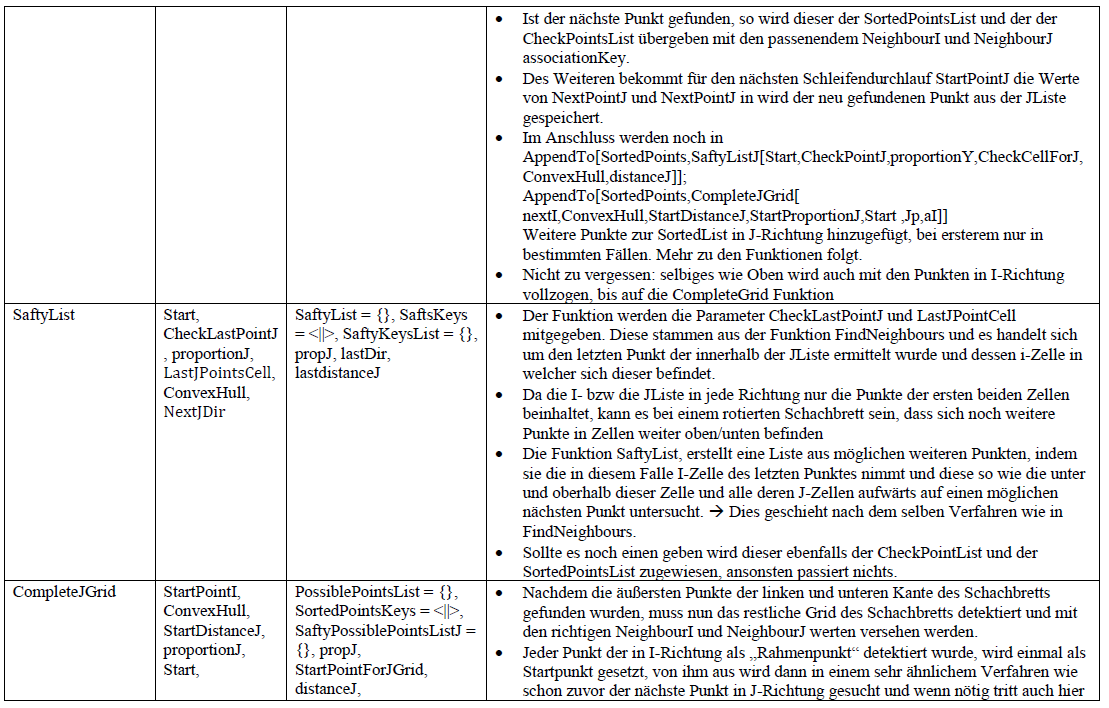
\includegraphics[width=1\linewidth]{images/KD4.png}
%	\captionof{figure}{Klassendiagramm}
%\end{minipage}
%\begin{minipage}{\linewidth}
%	\centering
%	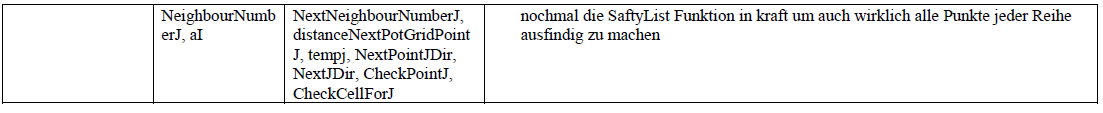
\includegraphics[width=1\linewidth]{images/KD5.png}
%	\captionof{figure}{Klassendiagramm}
%\end{minipage}\\


%Modulübersicht vllt in den Anhang??






